\chapter{Clearing The Window}
\label{chap:ClearWindow}

In this chapter we see all the steps that are required to clear our
window with a flat color.

During the application startup phase, we create some resources
required for rendering: two semaphores, used to synchronize the
execution of graphics and present commands, a command buffer,
used to submit commands to the GPU, and a render pass, used
to describe the rendering itself.

During the application main loop, we must follow these steps for our
rendering to be correct.
We acquire a swapchain image, this will be used as our render target.
Before starting recording new commands into the command buffer, we wait
for the previously submitted commands to finish their execution.
We bundle the acquired swapchain image into a framebuffer,
this will let us use said image during rendering.
We record the appropriate graphics commands into the command buffer.
We submit the command buffer to the graphics queue.
Finally, we submit a present command to the present queue.

\begin{figure}[ht]
    \centering
    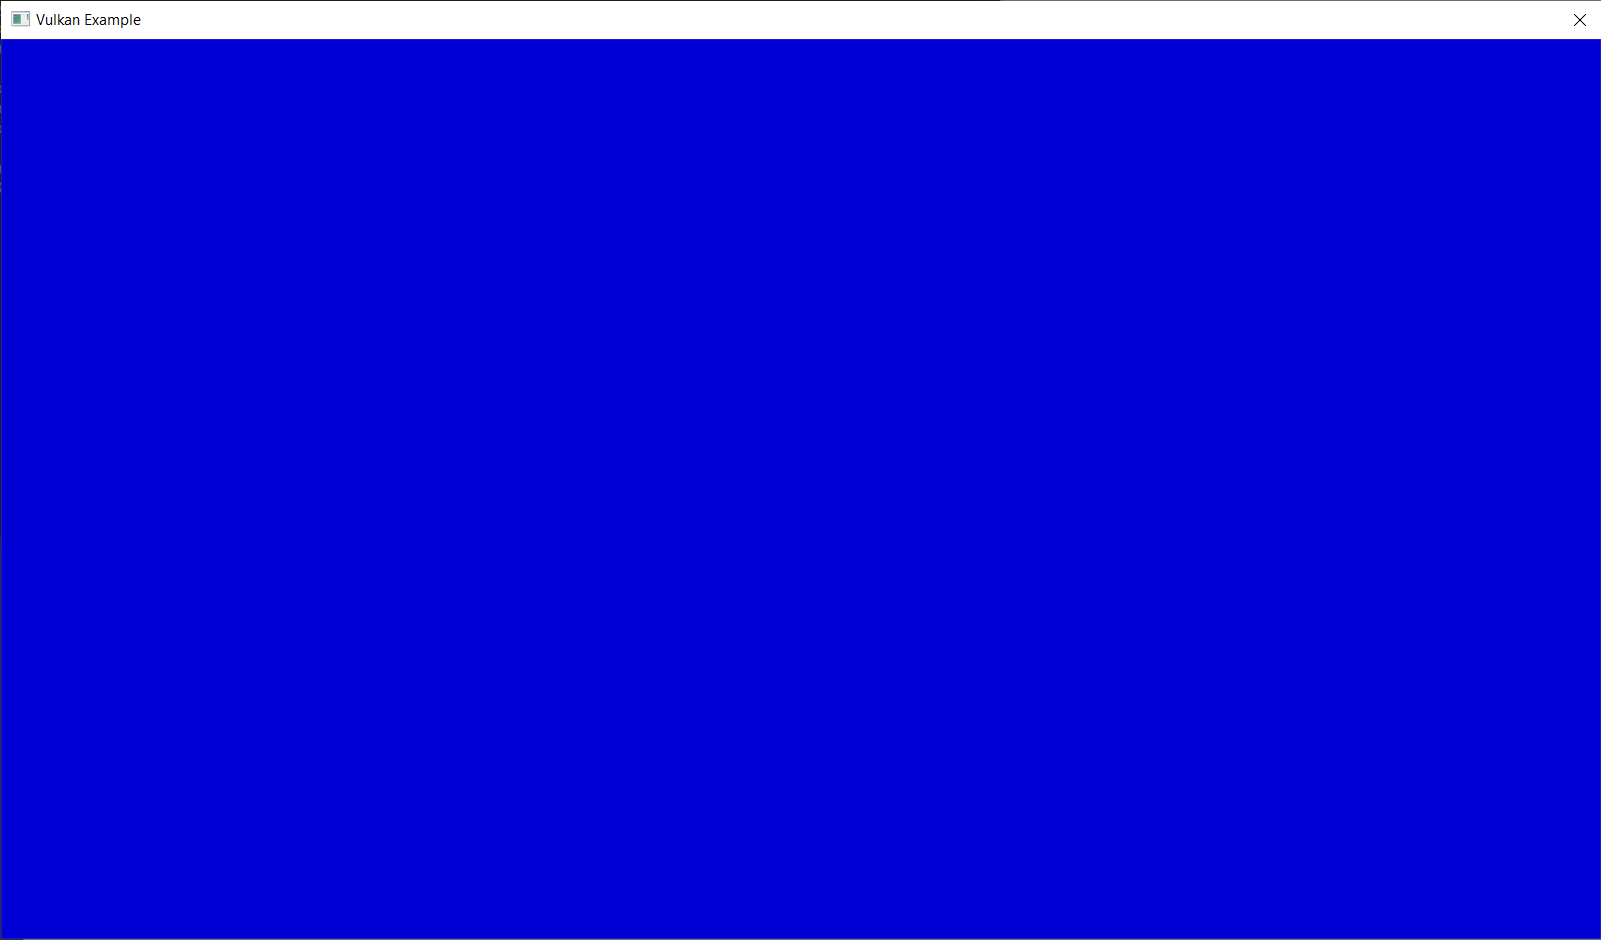
\includegraphics[scale=0.20]{images/ChClearWindow/ClearWindow.png}
    \caption{Clear the window background blue}
    \label{fig::ClearWindow}
\end{figure}

\section{Create Commands Synchronization Resources}

When we use Vulkan, we have to take into account the fact that we must
handle commands synchronizations ourselves.
In particular, we must synchronize rendering and present commands.
To accomplish this, we use two semaphores.
One semaphore will be signaled when a swapchain image is available to
be used as our render target.
When this semaphore is signaled, we may start rendering.
Another semaphore will be signaled when we finish rendering.
When this semaphore is signaled, we may present the image.

\begin{minipage}{\linewidth}{\noindent}
    \lstinputlisting[
        language=C++,
        caption={Create semaphores},
        label={lst::CreateSemaphores}
        ]{src/ChClearWindow/CreateSemaphores.cpp}
\end{minipage}

\subsection{Cleanup}

We destroy the previously allocated semaphores with \texttt{vkDestroySemaphore}.

\section{Create Command Buffer}

We use a command buffer to submit commands to the GPU.
We use \texttt{vkAllocateCommandBuffers} to create a command buffer.

\begin{minipage}{\linewidth}{\noindent}
    \lstinputlisting[
        language=C++,
        caption={Allocate a command buffer from our graphics command pool},
        label={lst::AllocateCommandBuffer}
        ]{src/ChClearWindow/AllocateCommandBuffer.cpp}
\end{minipage}

\subsection{VkCommandBufferAllocateInfo}

We use a \texttt{VkCommandBufferAllocateInfo} struct to configure the
command buffer we are about to create.
In our case we allocate a primary command buffer.
Such buffers can be directly submitted to the GPU; this is what we want.

\begin{minipage}{\linewidth}{\noindent}
    \lstinputlisting[
        language=C++,
        caption={Configure command buffer creation},
        label={lst::VkCommandBufferAllocateInfo}
        ]{src/ChClearWindow/VkCommandBufferAllocateInfo.cpp}
\end{minipage}

\subsection{Create Command Pool}

We create a command buffer allocating it from a command pool.
Thus, before creating a command buffer, we must create a command pool.
In our case, we explicitly submit commands only to the graphics queue.
Hence, we only need to create one graphics command pool.

\begin{minipage}{\linewidth}{\noindent}
    \lstinputlisting[
        language=C++,
        caption={Create graphics command pool},
        label={lst::CreateGraphicsCommandPool}
        ]{src/ChClearWindow/CreateGraphicsCommandPool.cpp}
\end{minipage}

\subsubsection{VkCommandPoolCreateInfo}

We use a \texttt{VkCommandPoolCreateInfo} struct to configure the command pool we are
about to create.
Here we use the reset command buffer flag because we want to be able to
write commands multiple times into the command buffers created from this pool.

\begin{minipage}{\linewidth}{\noindent}
    \lstinputlisting[
        language=C++,
        caption={Configure our graphics command pool},
        label={lst::VkCommandPoolCreateInfo}
        ]{src/ChClearWindow/VkCommandPoolCreateInfo.cpp}
\end{minipage}

\subsubsection{Cleanup}

When our application is shutting down, we have to destroy all the previously created
command pools.
To do this we use \texttt{vkDestroyCommandPool}.

\subsection{Command Buffer Fence}

Together with our command buffer, we also create a fence.
We can use a fence to wait for our command buffer execution to finish.
The fence that we create is already signaled from the start.
This is due to how we will use it later.

\begin{minipage}{\linewidth}{\noindent}
    \lstinputlisting[
        language=C++,
        caption={Create a fence for our command buffer},
        label={lst::CreateFence}
        ]{src/ChClearWindow/CreateFence.cpp}
\end{minipage}

\subsection{Cleanup}

We use \texttt{vkFreeCommandBuffers} to free the previously allocated command buffers.
We use \texttt{vkDestroyFence} to destroy our the previously created fences.

\section{Create Render Pass}

Before rendering, we need to describe what types of images will be used and the
order of our draw calls.
To do this we create a render pass.

\begin{minipage}{\linewidth}{\noindent}
    \lstinputlisting[
        language=C++,
        caption={Create a render pass},
        label={lst::CreateRenderPass}
        ]{src/ChClearWindow/CreateRenderPass.cpp}
\end{minipage}

\subsection{VkRenderPassCreateInfo}

We use a \texttt{VkRenderPassCreateInfo} struct to configure the render pass we
are about to create.

\begin{minipage}{\linewidth}{\noindent}
    \lstinputlisting[
        language=C++,
        caption={Configure our render pass},
        label={lst::VkRenderPassCreateInfo}
        ]{src/ChClearWindow/VkRenderPassCreateInfo.cpp}
\end{minipage}

\subsection{Render Pass Attachment Descriptions}

During render pass creation, we specify an array of attachment descriptions.
This array describes all the attachments that are going to be used by the
render pass.

In our case we have only one attachment.
This attachment will be one of the swapchain images.
We want to clear our attachment before using it for the first time in the
render pass.
We want to preserve the attachment's contents after using it for the last
time in the render pass.
We don't care about the attachment's stencil components.
We don't care about the attachment's image layout before starting the render pass.
We want to transition the attachment to a layout compatible with image presentation
at the end of the render pass.

\begin{minipage}{\linewidth}{\noindent}
    \lstinputlisting[
        language=C++,
        caption={Render pass attachment descriptions},
        label={lst::RenderPassAttachment}
        ]{src/ChClearWindow/RenderPassAttachments.cpp}
\end{minipage}

\subsection{Render Pass Subpasses}

During render pass creation, we specify an array of subpass descriptions.
This array describes the subpasses that define the render pass.

In our case we have only one subpass that uses our single attachment to write
color data into it.
Note that we specify the image layout that the attachment must have during
this subpass.

\begin{minipage}{\linewidth}{\noindent}
    \lstinputlisting[
        language=C++,
        caption={Render pass subpass descriptions},
        label={lst::RenderPassSubpasses}
        ]{src/ChClearWindow/RenderPassSubpasses.cpp}
\end{minipage}

\subsection{Cleanup}

To destroy our render pass we use \texttt{vkDestroyRenderPass}.

\section{Clear The Window}

In our application, for every iteration of the main loop, we render an image.
In this case, we simply clear the window background with a flat color.

\subsection{Acquire A Swapchain Image}

The first step for drawing something to the screen is to get an image that
serves as our render target.
This image must also be presentable to the presentation engine.
Only swapchain images satisfy the latter requirement.
Hence, we must use one of them as our render target.
The problem is that we don't know the next available swapchain image.
To determine such image we use \texttt{vkAcquireNextImageKHR}.
Note that the image is not guaranteed to be already available when
the function returns.
For this reason, we use the image available semaphore we created earlier.
It will be signaled when the image will actually be ready.

\begin{minipage}{\linewidth}{\noindent}
    \lstinputlisting[
        language=C++,
        caption={Acquire the next swapchain image that will be presented},
        label={lst::AcquireNextSwapchainImage}
        ]{src/ChClearWindow/AcquireNextSwapchainImage.cpp}
\end{minipage}

\subsection{Wait For The Previous Commands To Finish}

Before recording new commands into our command buffer, we have to wait
for the previously submitted commands to finish.
To do this wait on the command buffer fence.
After the wait terminates, we have to manually reset the fence state
to unsignaled.
We do this so that we can wait on the fence again, during the next frame.

\begin{minipage}{\linewidth}{\noindent}
    \lstinputlisting[
        language=C++,
        caption={Wait for command buffer execution to finish},
        label={lst::CommandBufferWait}
        ]{src/ChClearWindow/CommandBufferWait.cpp}
\end{minipage}

\subsection{Create A Framebuffer}

Before recording our rendering commands, we need to create a new framebuffer.
A framebuffer is the set of attachments that a render pass uses during rendering.
Before creating a new framebuffer, remember to destroy the framebuffer that was used
during the previous frame.
It's also important to remember to destroy the last created framebuffer during
the application cleanup phase.

\begin{minipage}{\linewidth}{\noindent}
    \lstinputlisting[
        language=C++,
        caption={Create a new framebuffer},
        label={lst::CreateFramebuffer}
        ]{src/ChClearWindow/CreateFramebuffer.cpp}
\end{minipage}

\subsubsection{VkFramebufferCreateInfo}

To configure the framebuffer we are about to create we use a
\texttt{VkFramebufferCreateInfo} struct.
In our case, our framebuffer will contain a single attachment: the next
available swapchain image.

\begin{minipage}{\linewidth}{\noindent}
    \lstinputlisting[
        language=C++,
        caption={Configure our framebuffer},
        label={lst::VkFramebufferCreateInfo}
        ]{src/ChClearWindow/VkFramebufferCreateInfo.cpp}
\end{minipage}

\subsection{Record Rendering Commands}

Now we can start recording the new rendering commands.
All the functions that write a command into our command buffer must lay
between \texttt{vkBeginCommandBuffer} and \texttt{vkEndCommandBuffer}.

\begin{minipage}{\linewidth}{\noindent}
    \lstinputlisting[
        language=C++,
        caption={Boilerplate code for recording a command buffer},
        label={lst::BeginEndCommandBuffer}
        ]{src/ChClearWindow/BeginEndCommandBuffer.cpp}
\end{minipage}

Here we are recording a one time submit command buffer.
It means that each recording will only be submitted once to the GPU.
Indeed, for every frame, we record and then submit our command buffer.
Hence, each recording will be submitted only once.
We do this so that we can change our clear color over time.

\begin{minipage}{\linewidth}{\noindent}
    \lstinputlisting[
        language=C++,
        caption={Change window clear color over time},
        label={lst::ComputeClearColor}
        ]{src/ChClearWindow/ComputeClearColor.cpp}
\end{minipage}

Now we can actually write some commands into our command buffer.
The idea is very simple.
We record two commands: the first is for starting an instance of our render pass;
the second is for ending the render pass instance.

\begin{minipage}{\linewidth}{\noindent}
    \lstinputlisting[
        language=C++,
        caption={Clear the window using a render pass},
        label={lst::RenderPassClearScreen}
        ]{src/ChClearWindow/RenderPassClearScreen.cpp}
\end{minipage}

First we have to configure the render pass instance using a \texttt{VkRenderPassBeginInfo}
struct.
The field that requires an explanation is \texttt{pClearValues}.
This is an array of clear values for each attachment.
The array is indexed by attachment number.
Consider the i-th attachment.
If it has \texttt{VK\_ATTACHMENT\_LOAD\_OP\_CLEAR}
as \texttt{loadOp} value, then \texttt{pClearValues[i]} will be used for the
clear value.
Otherwise, \texttt{pClearValues[i]} will be ignored.
We use the clear color we computed earlier as our clear value.

\begin{minipage}{\linewidth}{\noindent}
    \lstinputlisting[
        language=C++,
        caption={Configure our render pass instance},
        label={lst::VkRenderPassBeginInfo}
        ]{src/ChClearWindow/VkRenderPassBeginInfo.cpp}
\end{minipage}

Now we can explain how we clear the image with our clear value.
We start by beginning our render pass.
This causes the first subpass to start.
Right before the start of our subpass, an implicit image layout transition occurs.
This causes the swapchain image to transition to
\texttt{VK\_IMAGE\_LAYOUT\_COLOR\_ATTACHMENT\_OPTIMAL}.
With this layout, we can write color data into the image.
Since our subpass is the first to use our swapchain image color attachment, the image
is cleared using the specified clear value.
Right before ending the render pass, another implicit image layout transition occurs.
This causes the swapchain image to transition to
\texttt{VK\_IMAGE\_LAYOUT\_PRESENT\_SRC\_KHR}.
With this layout, our image can be used by the presentation engine.

\subsection{Submit Rendering Commands}

Once we have recorded all the necessary rendering commands into a command
buffer, we can submit it to the GPU for execution.
In our case, we submit the command buffer to the graphics queue.
When the execution of the command buffer is completed, our command buffer fence
will be signaled.

\begin{minipage}{\linewidth}{\noindent}
    \lstinputlisting[
        language=C++,
        caption={Submit command buffer to the GPU},
        label={lst::SubmitCommandBuffer}
        ]{src/ChClearWindow/SubmitCommandBuffer.cpp}
\end{minipage}

We use a \texttt{VkSubmitInfo} struct to configure our command buffer submission.

\texttt{pWaitSemaphores} is an array of semaphores upon which to wait before
the submitted command buffers begin execution.
In our case we only use one semaphore: our image available semaphore.
We do this because we have to wait for our swapchain image to be
available before rendering into it.

\texttt{pWaitDstStageMask} is a bitmask of pipeline stages at which
each corresponding semaphore wait will occur.
In our case we are saying that we do our semaphore wait as soon as the graphics
pipeline starts executing the commands recorded into our command buffer.

\texttt{pSignalSemaphores} is an array of semaphores to be signaled once
the submitted command buffers have completed execution.
In our case we signal only one semaphore: our render finished semaphore.
When this semaphore is signaled, it means that we have finished rendering our
image.

\begin{minipage}{\linewidth}{\noindent}
    \lstinputlisting[
        language=C++,
        caption={Configure command buffer submission},
        label={lst::VkSubmitInfo}
        ]{src/ChClearWindow/VkSubmitInfo.cpp}
\end{minipage}

\subsection{Present}

The only thing missing is to actually present our rendered image to the window.
Here we specify our present queue as the GPU queue that will execute our present
command.

\begin{minipage}{\linewidth}{\noindent}
    \lstinputlisting[
        language=C++,
        caption={Issue a present command},
        label={lst::Present}
        ]{src/ChClearWindow/Present.cpp}
\end{minipage}

We use a \texttt{VkPresentInfoKHR} struct to configure our present command submission.

\texttt{pWaitSemaphores} is an array of semaphores to wait for before issuing the present
command.
In our case we only use one semaphore: our render finished semaphore.
Simply put, we have to wait for our rendering to finish before presenting
the image to the window.

\begin{minipage}{\linewidth}{\noindent}
    \lstinputlisting[
        language=C++,
        caption={Configure present command submission},
        label={lst::VkPresentInfoKHR}
        ]{src/ChClearWindow/VkPresentInfoKHR.cpp}
\end{minipage}

\section{Cleanup}

Now that our application submits commands to the GPU, a problem may arise.
Being commands executed asynchronously on the GPU, we could exit the application,
and thus freeing all our resources, before all submitted commands finish
their execution.
This can lead to errors, because some commands may act upon one or more resources
that were deleted.
We can fix this issue by waiting for our device to be idle, meaning that
all processing on all device's queues is finished, before cleaning up our resources.
We can do this using \texttt{vkDeviceWaitIdle}.

\section{Our Application So Far}

Here we can see how all the concepts we have seen in this chapter come together
to form our application

\begin{minipage}{\linewidth}{\noindent}
    \lstinputlisting[
        language=C++,
        caption={Structure of our application},
        label={lst::ChClearWindowApp}
        ]{src/ChClearWindow/Application.cpp}
\end{minipage}
